\section{Conversione in formato SAM}

\subsection{Descrizione generale}
Come già detto, gli allineamenti ottenuti dallo Splice-Aware aligner sono in un formato non standard chiamato MEM, che contiene solo informazioni relative ai MEMs ottenuti in fase di allineamento. L'obiettivo di questa seconda parte è quello di convertire i due file MEM in un singolo file SAM\footnote{\url{http://samtools.github.io/hts-specs/SAMv1.pdf}} (Sequence Alignment Map), il formato standard per memorizzare gli allineamenti.

Il formato SAM è composto da 11 campi:

\begin{enumerate}
	\item \textbf{QNAME}: Il nome identificativo dell'allineamento
	\item \textbf{FLAG}: Una serie di flag binari che identificano le caratteristiche dell'allineamento
	\item \textbf{RNAME}: Identificativo del gene di riferimento
	\item \textbf{POS}: Posizione 1-based di inizio dell'allineamento sul genoma
	\item \textbf{MAPQ}:  Valore che indica la qualità dell'allineamento
	\item \textbf{CIGAR}: Stringa che identifica le operazioni effettuate per ottenere l'allineamento
	\item \textbf{RNEXT}: QNAME del mate (solo paired-end)
	\item \textbf{PNEXT}: POS del mate	(solo paired-end)
	\item \textbf{TLEN}:  Distanza tra mate (solo paired-end)
	\item \textbf{SEQ}:  	Allineamento vero e proprio
	\item \textbf{QUAL}: Valore che indica la qualità delle read
\end{enumerate}

Non si tratta solo di una semplice conversione, in quanto è necessario indurre diverse informazioni aggiuntive per avere un file SAM standard, quali: la posizione di inizio dell'allineamento sulla genomica, la stringa CIGAR, i flag relativi all'allineamento, ecc. Per supportare le read paired-end è stato necessario modificare gran parte di queste funzionalità. In particolare, è stata modificato il modo in cui vengono calcolati i campi FLAG, RNEXT, PNEXT e TLEN.

\newpage

\subsection{Computazione del campo FLAG per read paired-end}
Il campo FLAG è il secondo del formato SAM e consiste di un valore numerico (ottenuto convertendo in decimale una serie di flag binari) che rappresenta le caratteristiche dell'allineamento preso in esame. La seguente immagine mostra il significato di ciascun bit del flag:

\begin{figure}[h]
	\centering
	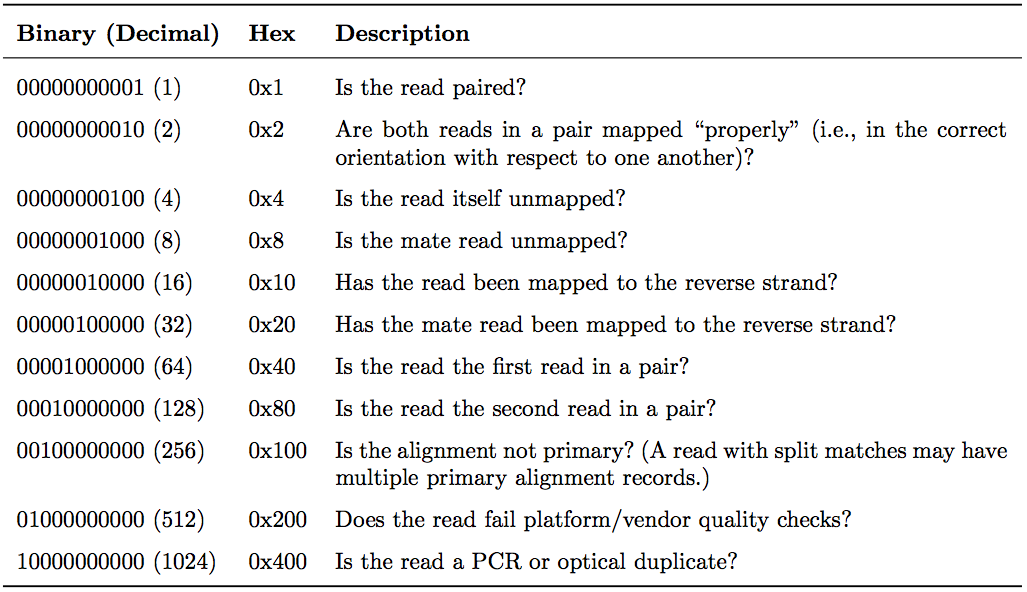
\includegraphics[width=\linewidth]{images/samflag.png}
  \caption{Il significato di ciascun bit del campo FLAG }
  \label{fig:SAM Flags}
\end{figure}

Nei casi single-end solo due flag vengono utilizzati: quello relativo allo strand (0x16) e quello relativo al tipo di allineamento (0x100); visto che le read non sono paired, il flag 0x1 sarà sempre false, quindi tutti i flag risultanti saranno pari.

Nei casi paired-end (quasi) tutti i flag vengono utilizzati. E' inoltre necessario trattare gli allineamenti a coppie, in quanto il campo FLAG esprime informazioni anche sul mate e non solo sull'allineamento preso in esame. 

Supponiamo ad esempio di avere due read, la prima che mappa sullo strand positivo e la seconda che non mappa (ed è quindi \textit{unmapped}). Sarà innanzitutto necessario mettere a true il flag relativo alle read paired-end (0x1) per entrambe le read. Considerando la prima, sarà messo a true il flag relativo al mate unmapped (0x8) e il flag relativo al first-in-pair (0x4). Considerando la seconda, sarà messo a true il flag relativo alla read unmapped (0x4) e quello relativo al second-in-pair(0x80). I flag in decimale saranno quindi 73 e 133.

Si noti che per il momento non viene tenuto conto dei flag 0x200 e 0x400, ma questo non è di alcuna rilevanza al fine di identificare eventi di Alternative Splicing.

\newpage

\subsection{Computazione dei campi RNEXT, PNEXT e TLEN}
I campi TLEN, RNEXT e PNEXT rappresentano rispettivamente il settimo, l'ottavo e il nono campo di ogni record del formato SAM; essi sono praticamente inutilizzati quando si allineano read single-end, ma nel formato paired-end assumono maggiore importanza. In particolare i campi RNEXT e PNEXT sono utilizzati da strumenti di visualizzazione degli allineamenti (come ad esempio IGV \cite{thorvaldsdottir2013integrative}) per permettere una corretta visualizzazione di una read e del suo mate.

Il campo RNEXT contiene il nome dell'allineamento relativo al mate (ovvero il suo campo PNAME). Per semplicità, quando i due allineamenti sono consecutivi, si può lasciare il suo valore a '='.

Il campo PNEXT contiene la posizione iniziale 1-based dell'allineamento relativo al mate (ovvero il suo campo POS. Qualora il mate fosse unmapped, si utilizza il valore 0.

Il campo TLEN rappresenta la distanza la lunghezza del template osservato, ovvero la distanza (sul genoma) tra l'inizio della prima read e la fine della seconda. Per la sua computazione è sufficiente trovare la posizione finale del secondo allineamento e sottrarre la posizione iniziale del primo.

La seguente immagine mostra un esempio di allineamento visualizzato da IGV:

\begin{figure}[h]
	\centering
	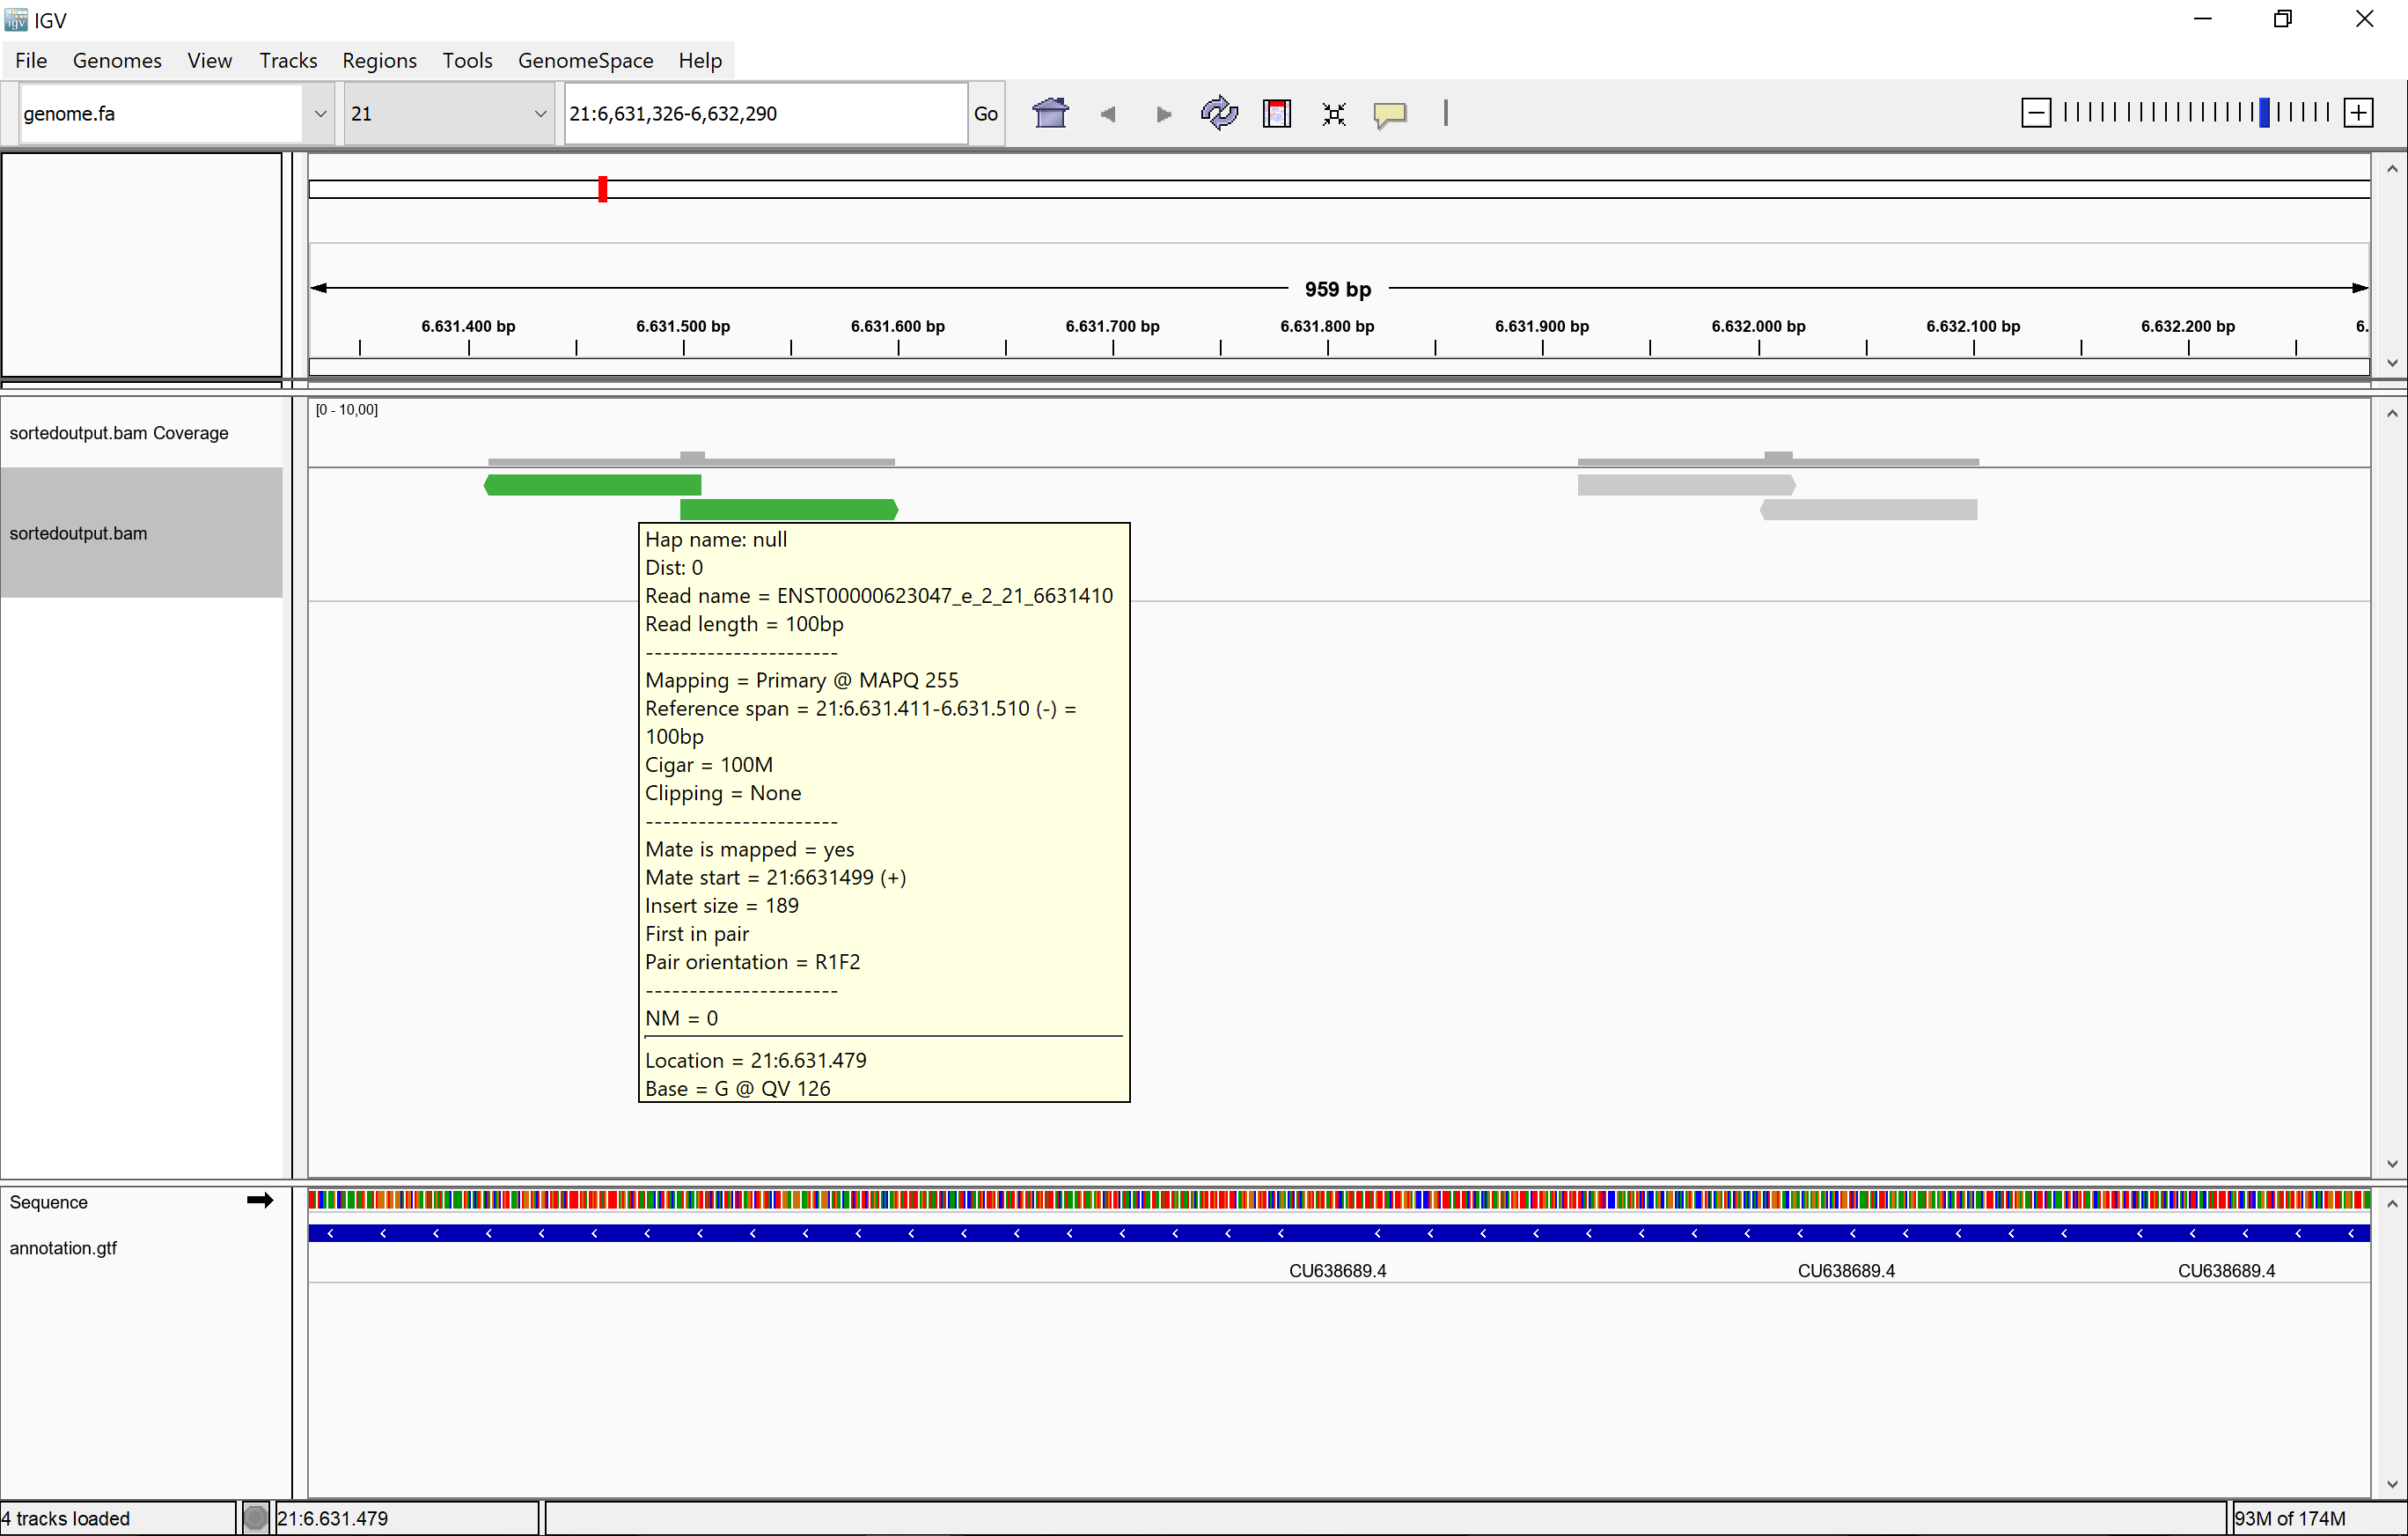
\includegraphics[width=\linewidth]{images/mateinfo.png}
  \caption{Informazioni sull'allineamento}
  \label{fig:MateInfo}
\end{figure}

\newpage

E' importante notare che, se questi campi sono settati correttamente, lasciando il cursore del mouse su un allineamento vengono visualizzate tutte le informazioni relative al mate. Al contrario, se si prova ad indicizzare il file BAM (la versione binaria del formato SAM) per l'utilizzo con IGV, e questi campi non sono stati settati correttamente, verrà visualizzato un errore. Un esempio errore è il seguente: se il campo FLAG non contiene 0x8 (quindi il mate è mapped), e si inserisce un valore di PNEXT diverso da 0, al momento dell'indicizzazione sarà visualizzato il messaggio "mapped mate cannot have zero coordinate; treated as unmapped".

\subsection{Calcolo delle statistiche dell'allineamento}
Seguendo l'esempio di altri allineatori (come ad esempio STAR), è stato deciso di visualizzare alcune statistiche in fase di allineamento, quali:

\begin{itemize}
	\item Numero di read mappate, non mappate e "placeholder"
	\item Numero di allineamenti primari e secondari
	\item IDMP medio
	\item TIDMP medio
\end{itemize}

Questi valori sono visualizzati nel file \textit{.alignsinfo.txt}. Anche se non hanno finalità particolari per la rilevazione di eventi di Alternative Splicing, essi forniscono uno strumento per valutare la qualità degli allineamenti effettuati da ASGAL.

\makeatletter
\newenvironment{CenteredBox}{% 
\begin{Sbox}}{% Save the content in a box
\end{Sbox}\centerline{\parbox{\wd\@Sbox}{\TheSbox}}}% And output it centered
\makeatother

\begin{figure}[thp]
\begin{CenteredBox}
  \begin{lstlisting}
Count mapped1: 1281/1313
Count mapped2: 1291/1295
Count unmapped reads1: 32
Count unmapped reads2: 4
Count placeholders1: 69
Count placeholders2: 87
Count mapped pairs: 1194
Count primary alignments: 958
Count secondary alignments: 236
Count one-side alignments: 184
Average idmp: 253.75795644891122
Average tidmp: 141.38358458961474
Average tlen: 915.1889352818372
  \end{lstlisting}
\end{CenteredBox}
\caption{Esempio di file \textit{.alignsinfo.txt}}
\end{figure}

%\begin{figure}[h!]
%	\centering
%	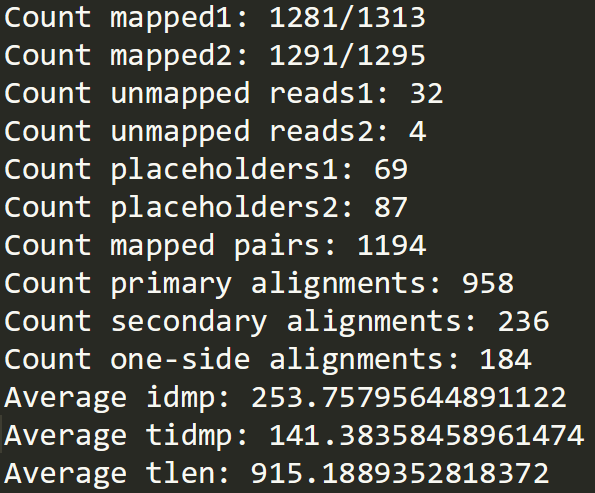
\includegraphics[height=5.5cm,width=8cm]{images/aligninfo.png}
%  \caption{Esempio di file \textit{.alignsinfo.txt}}
%  \label{fig:AlignsInfo}
%\end{figure}